\section{Tính toán hộp giảm tốc bánh răng nghiêng 1 cấp}
\subsection{Chọn vật liệu cho bánh dẫn và bánh bị dẫn}
Hộp giảm tốc chịu công suất không quá lớn nên chỉ cần chọn vật liệu có độ cứng HB $\leq$ 350.
\begin{itemize}
    \item Bánh dẫn: thép c45 tôi cải thiện 	Bánh dẫn: thép c45 tôi cải thiện đạt độ rắn HB 230…280 có $\sigma_{b1} = 850MPa; \sigma_{ch1} = 650MPa; HB_1 = 250$
    \item o	Bánh bị dẫn: thép c45 tôi cải thiện đạt độ rắn HB 192…240 có $\sigma_{b2} = 750MPa; \sigma_{ch2} = 450MPa; HB_2 = 235$
\end{itemize}
\subsection{Số chu kỳ làm việc cơ sở}
\begin{center}
        $N_{HO_1} = 30.HB_1^{2,4} = 30.250^{2,4} = 1,71.10^7$ chu kỳ \\
        $N_{HO_2} = 30.HB_2^{2,4} = 30.235^{2,4} = 1,47.10^7$ chu kỳ \\
        $N_{FO_1} = N_{FO_2} = 5.10^6$ chu kỳ \\
\end{center}
\subsection{Số chu kỳ làm việc tương đương, xác định theo sơ đồ tải trọng}
\begin{center}
    $N_{HE_1} = 60.c.n.L_h = 60.1.482,5.14400 = 41,69.10{-7}$ chu kỳ
\end{center}
Với c = 1; n = 482,5 vòng/phút; $L_h$= 6.300.8 = 14400 giờ. 
\begin{center}
    $N_{HE_2} = \frac{N_{HE_1}}{\mu} = \frac{41,69.10^7}{6,3} = 6,617.10^7$ chu kỳ
\end{center}
Tương tự:
\begin{center}
    $N_{FE_1} = 60.c.n.L_h = 60.1.76,6.14400 = 6,618.10^{-7}$ chu kỳ
\end{center}
\begin{center}
    $N_{FE_2} = \frac{N_{FE_1}}{\mu} = \frac{41,69.10^7}{6,3} = 6,617.10^7$ chu kỳ
\end{center} 
Vì $N_{HE_1} > N_{HO_1}; N_{HE_2} > N_{HO_2}; N_{FE_1} > N_{FO_1}; N_{FE_2} > N_{FO_2}$ \\
$\Rightarrow K_{HL_1} = K_{HL_2} = K_{FL_1} = K_{FL_2} = 1$
\subsection{Giới hạn mỏi tiếp xúc và giới hạn mỏi uốn}
\[
    \sigma_{OH_{lim}} = 2HB + 70 
\]
\[
    \Rightarrow \sigma_{OH_{lim1}} = 2.250 + 70 = 570MPa
\]
\[
    \Rightarrow \sigma_{OH_{lim2}} = 2.235 + 70 = 540MPa
\]
\[
    \sigma_{OF_{lim}} = 1.8HB
\]
\[
    \Rightarrow \sigma_{OF_{lim1}} = 1.8.250 = 450MPa
\]
\[
    \Rightarrow \sigma_{OF_{lim2}} = 1.8.235 = 423MPa
\]
\subsection{Ứng suất tiếp xúc cho phép}
\[
    [\sigma_{H}] = \frac{\sigma_{OH_{lim}}.Z_R.Z_V.Z_L.Z_XH}{s_H}.K_{HL} = \frac{\sigma_{OH_{lim}}.0,9}{s_H}.K_{HL}
\]
Khi tôi cải thiện $s_H = 1,1$, do đó:
\[
    [\sigma_{H_1}] = \frac{570.0,9}{1,1}.1 = 466,37MPa
\]
\[
    [\sigma_{H_2}] = \frac{540.0,9}{1,1}.1 = 441,82MPa
\]
Ứng suất tính toán cho phép:
\[
    [\sigma_H] = 0,45.([\sigma_{H1}] + [\sigma_{H2}]) = 0,45.(466,37 + 441,82) = 408,68MPa
\]
Tuy nhiên
\[
    [\sigma_{min}] \leq [\sigma_H] \leq 1,25[\sigma_{min}] \Leftrightarrow 441.82 \leq [\sigma_H] \leq 552,275
\]
$\Rightarrow$ Ta chọn $[\sigma_H] = [\sigma_{H2}] = 441,82$ MPa
\subsection{Ứng suất uốn cho phép}
\[
    [\sigma_F] =\frac{\sigma_{OFlim}}{s_F}.K_{HL}
\]
Chọn $s_F = 1,75$, ta có: \\
\[
    [\sigma_{F1}] =\frac{\sigma_{OF1lim}}{s_F}.K_{HL} = \frac{450}{1,75}.1 = 257,143 (MPa)
\]
\[
    [\sigma_{F2}] =\frac{\sigma_{OF2lim}}{s_F}.K_{HL} = \frac{423}{1,75}.1 = 241,7 (MPa)
\]
\subsection{Khoảng cách trục}
Do bánh răng nằm đối xứng các ổ trục nên $\Psi_{ba} = 0,3 \div 0,5$, chọn $\Psi_{ba} = 0,4$ \\
Khi đó $\Psi_{bd} = \frac{\Psi_{ba}.(u+1)}{2} = \frac{0,4.(6,3+1)}{2} = 1,46$ \\
Từ đó tra theo bảng 6.4 ta chọn: $K_{H\beta} = 1,07$, $K_{F\beta} = 1,14$ \\
Tính khoảng cách trục: \\
\[
    a_w = 500.(u+1).\sqrt[3]{\frac{T_1.K_{H\beta}}{\Psi_{ba}.[\sigma_H]^2.u}} = 500.(6,3+1).\sqrt[3]{\frac{63,73.1,07}{0,4.408,68^2.6,3}} = 198,98 (mm)
\]
Theo tiêu chuẩn ta chọn $a_w = 200mm$
\subsection{Môđun răng}
\[
    m_n = (0,01 \div 0,02).a_w = 2 \div 4
\]
Theo tiêu chuẩn ta chọn $m_n = 4$
\subsection{Số răng}
Từ điều kiện $20^\circ \leq \beta \leq 8^\circ$ \\
\[
    \Leftrightarrow \frac{2.a_w.\cos8^\circ}{m_n.(u+1)} \leq z_1 \leq \frac{2.a_w.\cos20^\circ}{m_n.(u+1)}
\]
\[
    \Leftrightarrow \frac{2.200.\cos8^\circ}{4.(6,3+1)} \leq z_1 \leq \frac{2.200.\cos20^\circ}{4.(6,3+1)}
\]
\[
    \Leftrightarrow 13,56 \leq z_1 \leq 12,87
\]
$\Rightarrow$ Chọn $z_1 = 13 \Rightarrow z_2 = u.z_1 = 6,3.13 = 81,9$ \\
$\Rightarrow$ Chọn $z_2 = 82$ \\
Góc nghiêng răng: 
\[
    \beta = \arccos\frac{m_n.(z_1+z_2)}{2.a_w} = \arccos\frac{4.(13+82)}{2.200} = 18,2^\circ
\]
\subsection{Tỉ số truyền sau khi chọn răng}
\[
    u = \frac{z_2}{z_1} = \frac{82}{13} = 6,308
\]
\subsection{Các thông số hình học}
Đường kính vòng chia: \\
\[
    d_1 = \frac{m_n.z_1}{\cos\beta} = \frac{4.13}{\cos18,2^\circ} = 54,738 (mm)
\]
\[
    d_2 = \frac{m_n.z_2}{\cos\beta} = \frac{4.82}{\cos18,2^\circ} = 345,27 (mm)
\]
Đường kính vòng đỉnh: \\
\[
    d_{a1} = d_1 + 2.m_n = 54,738 + 2.4 = 62,738 (mm)
\]
\[
    d_{a2} = d_2 + 2.m_n = 354,27 + 2.4 = 362,27 (mm)
\]
Đường kính vòng đáy: \\ 
\[
    d_{f1} = d_1 - 2,5m_n = 62,738 - 2,5.4 = 44,738 (mm)
\]
\[
    d_{f2} = d_2 - 2,5m_n = 345,27 - 2,5.4 = 335,27 (mm)
\]
Tính lại khoảng cách trục: \\
\[
    a_w = \frac{m_n.(z_1+z_2)}{2\cos\beta} = \frac{4.(13+82)}{2.\cos18,2^\circ} = 200(mm)
\]
Chiều rộng vành răng: 
\begin{itemize}
    \item Bánh bị dẫn: $b_2 = \Psi_{ba}.a_w = 0,4.200 = 80(mm)$
    \item Bánh dẫn: $b_1 = b_2 + 5 = 85(mm)$
\end{itemize}
\subsection{Vận tốc vòng bánh răng}
\[
    v = \frac{\pi.d_1.n_1}{60000} = \frac{\pi.54,738.482,5}{60000} = 1,38 (m/s)
\]
Theo bảng 6.3 ta chọn cấp chính xác 9 với $v_{gh} = 6 m/s$
\subsection{Tính toán kiểm nghiệm giá trị ứng suất tiếp xúc}
Theo bảng 6.6 ta chọn hệ số tải trọng động $K_{HV} = 1,11$, $K_{FV} = 1,22$ \\
\[
    \sigma_H = \frac{z_M.z_H.z_\epsilon}{d_1}.\sqrt{\frac{2.T_1.10^3.K_{H\beta}.K_{HV}.(u+1)}{b_w.u}} 
\]
\[
    = \frac{190.2,3847.0,8124}{54,738}.\sqrt{\frac{2.63,73.10^3.1,07.1,11.(6,3+1)}{80.6,3}} = 314,887 (MPa)
\]
Với:
\begin{itemize}
    \item $Z_M = 190$ vì vật liệu bằng thép
    \item $Z_H = \sqrt{\frac{4.\cos\beta}{\sin(2.\alpha_{tw})}} = \sqrt{\frac{4.\cos18,2}{\sin(2.20,9637)}} = 2,3847$
    \item $\alpha_{tw} = \arctan(\frac{\tan\alpha_{nw}}{\cos\beta}) = \arctan(\frac{\tan20}{\cos18,2}) = 20,9637$
    \item $Z_\epsilon = \sqrt{\frac{1}{\epsilon_\alpha}} = \sqrt{\frac{1}{1,515}} = 0,8124$
    \item $\epsilon_\alpha = [1,88-3,2.(\frac{1}{z_1}+\frac{1}{z_2})].\cos\beta = [1,88-3,2.(\frac{1}{13}+\frac{1}{82})].\cos18,2 = 1,515$
\end{itemize}
\[
    \sigma_H = 314,887 MPa \leq 441,82 MPa
\]
    $\Rightarrow \sigma_H \leq [\sigma_H]$ thỏa mãn\\
\subsection{Số răng tương đương}
\[
    z_{v1} = \frac{z_1}{\cos^3(\beta)} = \frac{13}{\cos^3(18,2)} = 13,685 \Rightarrow z_{v1} = 14
\]
\[
    z_{v2} = \frac{z_2}{\cos^3(\beta)} = \frac{82}{\cos^3(18,2)} = 86,32 \Rightarrow z_{v1} = 87
\]
\subsection{Hệ số dạng răng}
\begin{itemize}
    \item Đối với bánh dẫn: $Y_{F1} = 3,47 + \frac{13,2}{z_{v1}} = 3,47 + \frac{13,2}{14} = 4,413$
    \item Đối với bánh bị dẫn: $Y_{F2} = 3,47 + \frac{13,2}{z_{v2}} = 3,47 + \frac{13,2}{87} = 3,622$
\end{itemize}
\subsection{Ứng suất uốn tính toán}
Đặc tính so sánh độ bền uốn:
\begin{itemize}
    \item Bánh dẫn: $\frac{[\sigma_{F1}]}{Y_{F1}} = \frac{257,143}{4,413} = 58,27$
    \item Bánh bị dẫn: $\frac{[\sigma_{F2}]}{Y_{F2}} = \frac{241,7}{3,622} = 66,73$
\end{itemize}
$\Rightarrow$ Ta kiểm tra độ bền uốn theo bánh dẫn có độ bền thấp hơn:\\
Ứng suất uốn tính toán:
\[
    \sigma_{F1} = \frac{Y_{F1}.F_t.K_{F1}.Y_\epsilon.Y_\beta}{b_2.m} = \frac{4,413.2328,547.1,39.0,66.0,6985}{80.4} = 20,577 (MPa)
\] 
Với: 
\begin{itemize}
    \item $Y_\epsilon = \frac{1}{\epsilon_\alpha} = \frac{1}{1,515} = 0,66$
    \item $F_t = 2.10^3.\frac{T_1}{d_{w1}} = 2.10^3.\frac{63,73}{54,738} = 2328,547$
    \item $Y_\beta = 1 - \epsilon_\beta\frac{\beta}{120} = 1 - 1,988\frac{18,2}{120} = 0,6985$
    \item $\epsilon_\beta = b_w.\frac{\sin\beta}{\pi.m} = 80.\frac{\sin18,2}{\pi.4} = 1,988$
    \item $K_{F1} = K_{F\alpha}.K_{F\beta}.K_{FV} = 1.1,14.1,22 = 1,39$
    \item $K_{F\alpha} = \frac{4 + (\epsilon_\alpha - 1).(n_{cx} - 5)}{4\epsilon_\alpha} = \frac{4 + (1,515 - 1).(9 - 5)}{4.1,515} = 1$
\end{itemize}
$\Rightarrow \sigma_{F1} < [\sigma_{F1}] = 257,143$ MPa do đó độ bền uốn thỏa\\
\subsection{Phân tích lực}
\begin{figure}[H]
    \centering
    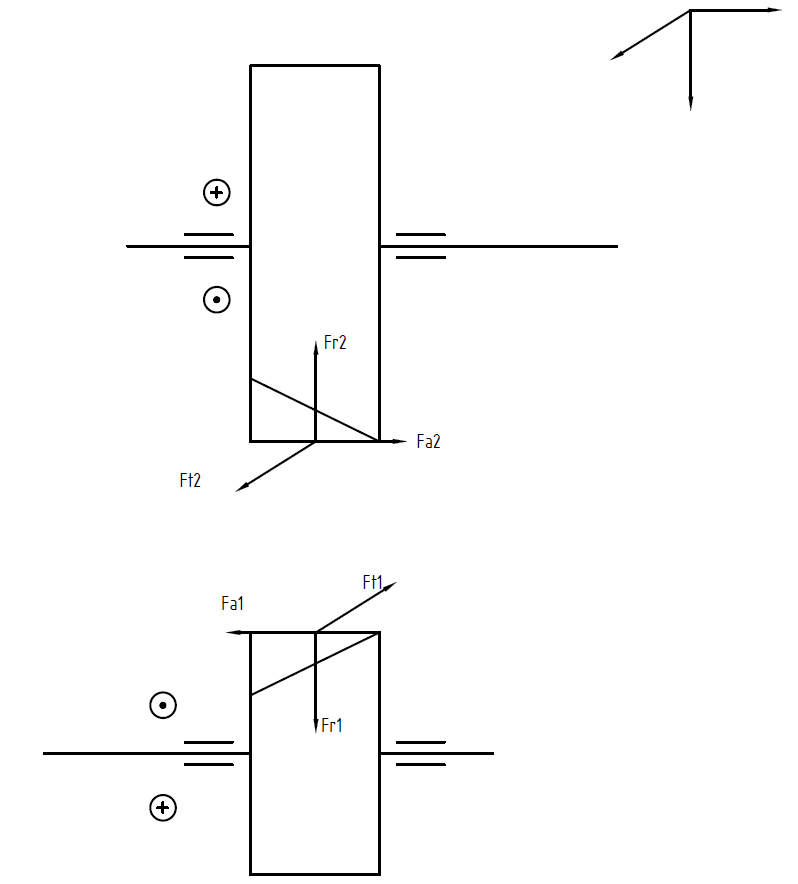
\includegraphics[width=0.5\textwidth]{pictures/phantichluc.png}
\end{figure}
\cleardoublepage